\chapter{Utility Maximization}

\section{Consumer Preferences}

\begin{itemize}
    \item $X$: consumption set
    \item $\mathbf x$: consumption bundle
\end{itemize}

\block{Definition}{
    \begin{enumerate}
        \item $\succsim$: weak preference  
        \item $\succ$: strict preference  
        \item $\sim$: indifference  
    \end{enumerate}
}

\block{Theorem}{
    \begin{enumerate}
        \item \textbf{Complete} (完整性): For all $\mathbf x$ and $\mathbf y$ in $X$, either $\mathbf x \succsim y$ or $\mathbf y \succsim \mathbf x$ or both. (兩個消費組合可比較)
        \item \textbf{Reflexive} (反身性): For all $\mathbf x$ in $X$, $\mathbf x \succsim \mathbf x$. (至少跟自己一樣好)
        \item \textbf{Transitive} (遞移性): For all $\mathbf x$, $\mathbf y$, and $z$ in $X$, if $\mathbf x \succsim \mathbf y $ and $\mathbf \mathbf y \succsim \mathbf z$, then $\mathbf x \succsim \mathbf z$.  
        \item \textbf{Continuity} (連續性): For all $\mathbf y$ in $X$, the sets $\{\mathbf x: \mathbf x \succsim \mathbf y\}$ and $\{\mathbf x:\mathbf x \precsim \mathbf y\}$ are closed sets. It follows that $\{\mathbf x: \mathbf x \succ \mathbf y \}$ and $\{ \mathbf x: \mathbf x \prec \mathbf y \}$ are open sets.  
    \end{enumerate}
}

\block{Definition: Utility Function}{
It is often convenient to summarize a consumer’s behavior by means of a \textbf{utility function}; that is, a function $u: X \to \mathbb{R}$ such that $\mathbf x \succ \mathbf y \iff u(\mathbf x) > u(\mathbf y)$. 
It can be shown that if the preference ordering is \highlight{complete, reflexive, transitive, and continuous}, then it can be represented by a continuous utility function.
}
\noindent The only relevant feature of a utility function is its ordinal character. 
If $u(\mathbf{x})$ represents some preferences $\succsim$ and $f: \mathbb{R} \to \mathbb{R}$ is a monotonic function, then $f(u(\mathbf{x}))$ will represent exactly the same preferences since $f(u(\mathbf{x})) \geq f(u(\mathbf{y}))$ if and only if $u(\mathbf{x}) \geq u(\mathbf{y})$.  

\block{Theorem}{
    Some assumptions on preferences:
    \begin{enumerate}
    \item \textbf{Weak monotonicity}: If $\mathbf x \geq \mathbf y$, then $\mathbf x \succsim \mathbf y$.  

    At least as much of everything is at least as good.  

    \item \textbf{Strong monotonicity}: If $\mathbf x \geq \mathbf y$ and $\mathbf x \neq \mathbf y$, then $\mathbf x \succ \mathbf y$.  

    At least as much of every good, and strictly more of some good, is strictly better. This is simply assuming that goods are good.  

    \item \textbf{local nonsatiation}: Given any $\mathbf x$ in $X$ and any $\epsilon > 0$, there is some bundle $y$ in $X$ with $\|\mathbf x - \mathbf y\| < \epsilon$ such that $\mathbf y \succ \mathbf x$.  

    Local nonsatiation says that one can always do a little bit better, even if one is restricted to only small changes in the consumption bundle. You should verify that \highlight{strong monotonicity implies local nonsatiation but not vice versa}. Local nonsatiation rules out "thick" indifference curves.  

    \item \textbf{Convexity}: Given $\mathbf{\mathbf x}$, $\mathbf{\mathbf y}$, and $\mathbf{\mathbf z}$ in $X$ such that $\mathbf{\mathbf x} \succsim \mathbf{\mathbf z}$ and $\mathbf{\mathbf y} \succsim \mathbf{\mathbf z}$, then it follows that $t\mathbf{\mathbf x} + (1-t)\mathbf{\mathbf y} \succsim \mathbf{\mathbf z}$ for all $0 \leq t \leq 1$.  

    \item \textbf{Strict Convexity}: Given $\mathbf{\mathbf x} \neq \mathbf{\mathbf y}$, and $\mathbf{\mathbf z}$ in $X$ such that $\mathbf{\mathbf x} \succsim \mathbf{\mathbf z}$ and $\mathbf{\mathbf y} \succsim \mathbf{\mathbf z}$, then it follows that $t\mathbf{\mathbf x} + (1-t)\mathbf{\mathbf y} \succ \mathbf{\mathbf z}$ for all $0 < t < 1$.  
    
    Convexity implies that an agent prefers averages to extremes, but, other than that, it has little economic content.
    \end{enumerate}
}



\block{Example: The existence of a utility function}{
    Skip.
}

\block{Example: The marginal rate of substitution}{
    Let $u(x_1, \dots, x_k)$ be a utility function. Suppose that we increase the amount of good $i$; how does the consumer have to change his consumption of good $j$ in order to keep utility constant?  

    We let $dx_i$ and $dx_j$ be the changes in $x_i$ and $x_j$.
    By assumption, the change in utility must be zero, so 
    \[
        \frac{\partial u(\mathbf{x})}{\partial x_i}dx_i + \frac{\partial u(\mathbf{x})}{\partial x_j}dx_j = 0
    \]

    Hence,  
    \[
        \frac{dx_j}{dx_i} = 
        -
        \frac{v^\prime(u) \frac{\partial u(\mathbf{x})}{\partial x_i}}{v^\prime(u)
        \frac{\partial u(\mathbf{x})}{\partial x_j}} =
        -
        \frac{ \frac{\partial u(\mathbf{x})}{\partial x_i}}{
        \frac{\partial u(\mathbf{x})}{\partial x_j}}
    \]
    This is known as the marginal rate of substitution between good $i$ and $j$.
}


\section{Consumer Behavior}


Let 
\begin{itemize}
    \item $m$ be the fixed amount of money available to be a consumer
    \item $\mathbf{p} = (p_1, \dots, p_k)$ be the vector of prices of goods, $1, \dots, k$
\end{itemize}
The set of affordable bundles, the budget set of the consumer, is given by
\[
    B = \{ \mathbf{x} \in X : \mathbf{px} \leq m \}.
\]
The problem of preference maximization can then be written as:

\begin{equation*}
    \begin{array}{rl}
        \max & \quad u(\mathbf{x}) \\
        \text{s.t.} & \quad \mathbf{px} \leq m
    \end{array} \longrightarrow
    \begin{array}{rl}
        & \quad \mathbf{x} \in X \\
        \max & \quad u(\mathbf{x}) \\
        \text{s.t.} & \quad \mathbf{px} = m.
    \end{array}
\end{equation*}



\begin{enumerate}
    \item We need to verify that the objective function is continuous and that the constraint set is closed and bounded.
    \item We examine concerns the representation of preferences.  
    Here we can observe that the maximizing choice $\mathbf{x}^*$ will be independent of the choice of utility function used to represent the preferences.
    \item If we multiply all prices and income by some positive constant, we will not change the budget set, and thus we cannot change the set of optimal choices. 
    \[
        \begin{array}{l}    
            \mathbf{x}^* \succeq \mathbf{x} \quad \forall \mathbf{x} \\
            \text{s.t.} \quad \mathbf{px} \leq m
        \end{array}
        \implies 
        \begin{array}{l}    
            \mathbf{x}^* \succeq \mathbf{y} \quad \forall \mathbf{y} \\
            \text{s.t.} \quad \mathbf{tpx} \leq tm
        \end{array}
    \]
    (The optimal choice set, $\mathbf{x}^*$, is HD-0 in price, $\mathbf{p}$ , and income, $m$.)
\end{enumerate}

According to the local nonsatiation hypothesis, there must be some bundle $\mathbf{x}$ which is close to and prefer to $\mathbf{x}^*$.
But this meands that $\mathbf{x}^*$ could not maximize preference on the budget set B. 
Therefore, under the local nonsatiation assumption, a utility-maximizing bundle $\mathbf{x}^*$ must meet the budget constraint with equality.
This allows us to restate the consumer's problem as
\begin{align*}
    v(\mathbf{p}, m) = \max & \quad u(\mathbf{x}) \\
    \text{s.t.} & \quad \mathbf{px} = m.
\end{align*}
\block{Definition: Indirect Utility Function}{
    The function $v(\mathbf{p}, m)$ that gives us the maximum utility achievable at given prices and income is called the \textbf{indirect utility function}. 
    (給定價格與收入,求最大效用)
}
\block{Definition: Demand Function}{
    The consumer's \textbf{demand function} is given  by the $\mathbf{x} (\mathbf{p}, m)$.
    It expresses how much of each good the consumer desires at a given level of prices and income.
}
\block{Theorem}{
    We need to make a few assumptions to make sure that this demand function is well-defined:
    \begin{enumerate}
        \item Unique bundle that maximizes utility (strict convexity).
        \item Demand function is HD-0 in $(\mathbf{p}, m)$.
        \item Utility function is differentiable. ??
    \end{enumerate}
}
As long as the utility function is differentiable, the Lagrangian for the utility maximization problem can be written as
\begin{align*}
    \mathcal{L} =& u(\mathbf{x}) - \lambda (\mathbf{px} - m) \\
    \implies & \frac{\partial u(\mathbf x)}{\partial x_i} -\lambda p_i = 0 \quad \text{for } i =1, \dots, k \\
    \implies & \frac{\frac{\partial u(\mathbf{x})}{\partial x_i}}{\frac{\partial u(\mathbf{x})}{\partial x_j}} = \frac{p_i}{p_j} \quad \text{for } i,j = 1, \dots, k
\end{align*}
The fraction on the left is the MRS between good $i$ and $j$, and the fraction on the right might be called the \textbf{economic rate of substitution between good $i$ and $j$.} 
\highlight{Maximization imp-}
\highlight{lies that these two rates of substitution be equal}.

\begin{figure}[H]
    \center
    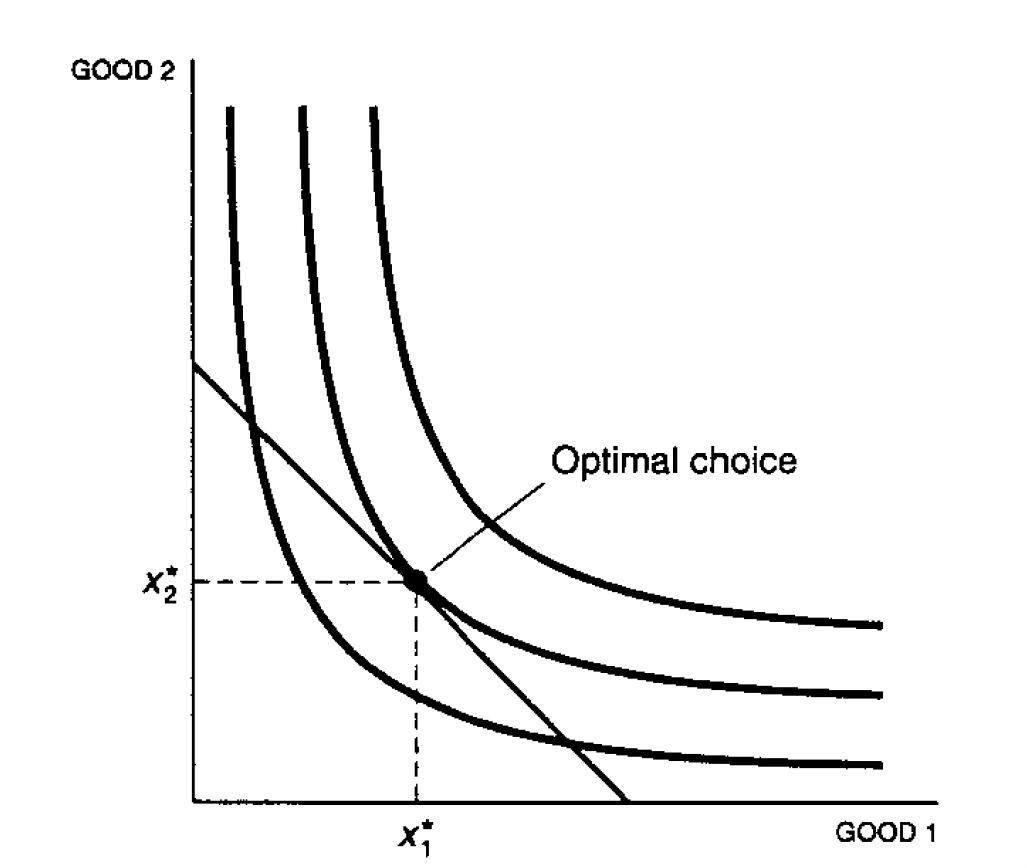
\includegraphics[scale=0.5]{img/fig8-1.png}
    % \caption{Waterloo, ON}
\end{figure}
\begin{itemize}
    \item Budget line: $\{ \mathbf{x} : p_1x_1 + p_2x_2 = m \} \to x_2 = \frac{m}{p_2} - \left( \frac{p_1}{p_2} \right)x_1.$
    \begin{itemize}
        \item Vertical intercept: $\frac{m}{p_2}$
        \item Slope: $-\frac{p_1}{p_2}$
    \end{itemize}
\end{itemize}
The slope of the indifference curve equals the slope of the budget line.  
The optimal consumption bundle happens at the tangent point.

Let $\mathbf{x}^*$ be an optimal choice, and let $\mathbf{dx}$ be a perturbation of $\mathbf{x}^*$ that satisfies the budget constraint. Hence, we must have
\[
    \mathbf{p(x^* \pm dx)} = m.
\]
Since $\mathbf{px} = m$, this equation implies that $\mathbf{p \ dx} = 0$, which in turn implies that $\mathbf{dx}$ must be orthogonal to $\mathbf{p}$.  
For any such perturbation $\mathbf{dx}$, utility cannot change, or else $\mathbf{x}^*$ would not be optimal. 
Hence, we have
\[
\mathbf{D}u(\mathbf{x}^*)\mathbf{dx} = 0.
\]
It in turn implies that:

\begin{enumerate}
    \item $\mathbf{Du}(\mathbf{x}^*)$ must be orthogonal to $\mathbf{dx}$.
    \item $\mathbf{Du}(\mathbf{x}^*)$ must be proportional to $\mathbf{dx}$.
\end{enumerate}

The second derivative of the Lagrangian with respect to goods $i$ and $j$ is $\frac{\partial^2 u(\mathbf{x})}{\partial x_i \partial x_j}$. Hence, the second-order condition can be written as
\[
\mathbf{h}^t \mathbf{D}^2 u(\mathbf{x}^*) \mathbf{h} \leq 0 \quad \forall \ h \ \text{such that} \ \mathbf{ph} = 0.
\]
This condition requires that the Hessian matrix of the utility function is \highlight{negative semidefinite} for all vectors $\mathbf{h}$ orthogonal to the price vector.


\section{Indirect Utility}

\block{Theorem: Indirect Utility Function}{
    Properties of the indirect utility function:
    \begin{enumerate}
        \item $v(\mathbf p, m)$ is nonincreasing in $\mathbf p$; that is, if $\mathbf p^\prime \geq \mathbf p$, $v(\mathbf p^\prime, m) \leq v(\mathbf p, m)$. Similarly, $v(\mathbf p, m)$ is nondecreasing in $m$.
        \item $v(\mathbf p, m)$  is HD-0 in $(\mathbf p, m)$.
        \item $v(\mathbf p, m)$ is a quasi-convex in $\mathbf p$; that is $\{ \mathbf p :v(\mathbf p, m) \leq k \}$ is a convex set for all $k$.
        \item $v(\mathbf p, m)$ is continuous at all $\mathbf p \gg 0, m >0$.
    \end{enumerate}
}

\begin{figure}
    \center
    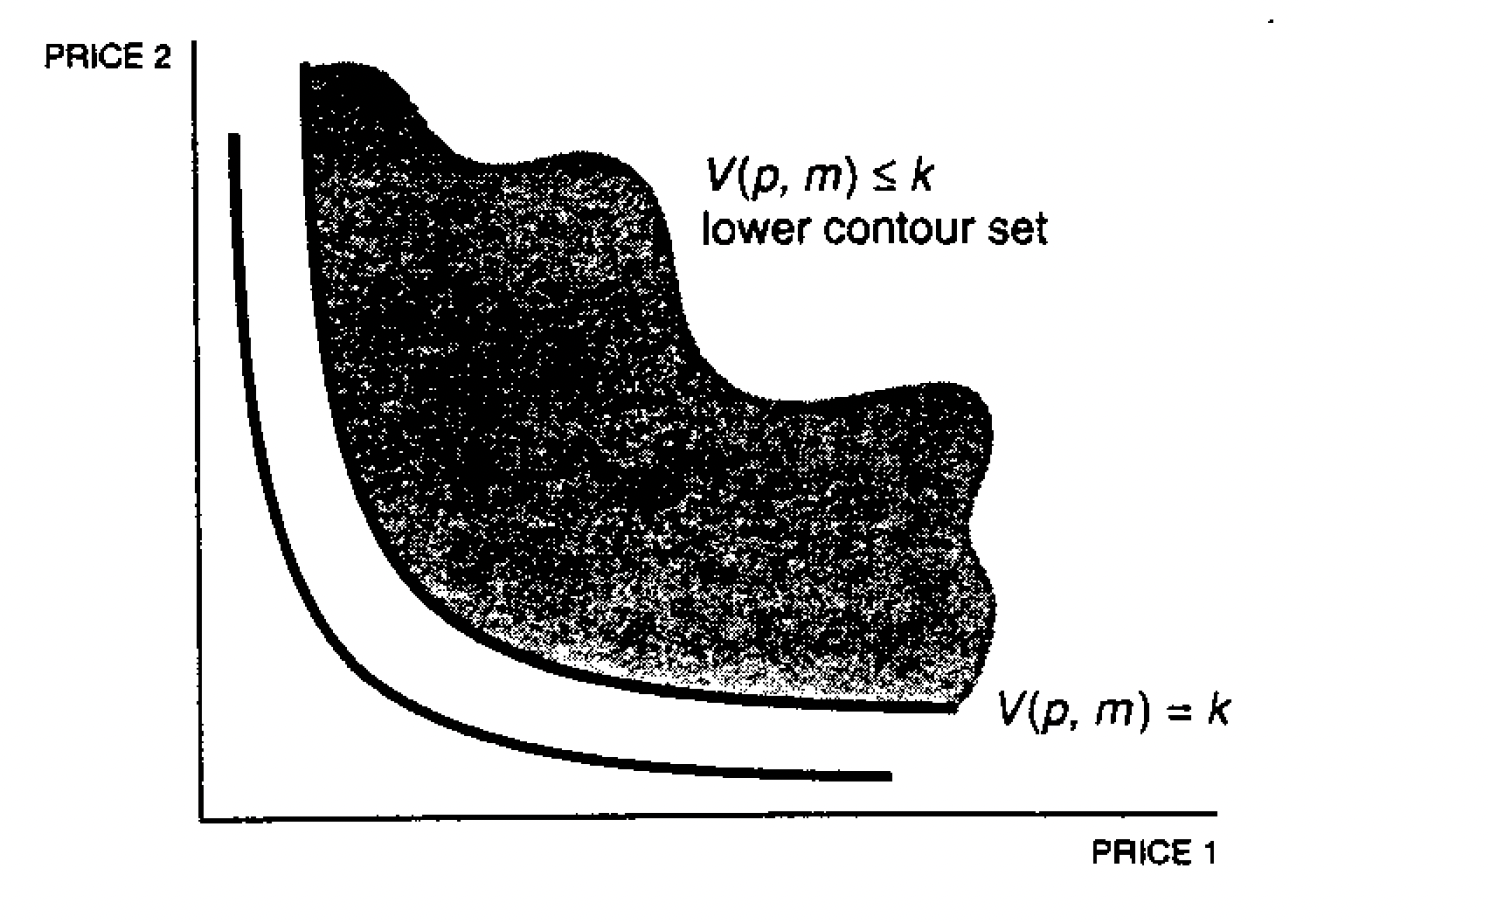
\includegraphics[width=0.7\textwidth]{img/fig7-2}
    \caption{}
\end{figure}

If preference satisfy the local nonsatiation assumption, then $v(\mathbf{p}, m)$ will be strictly increase in $m$. 
Since $v(\mathbf{p}, m)$ is strictly increase in $m$, we can convert the function and solve for $m$ as a function of the level of utility $u$.
That is, given any level of utility, $u$, we can get the minimal amount of income necessay to achieve utility $u$ at price $p$.
The \highlight{inverse of t-}
\highlight{he indirect utility function is known as the \textbf{expenditure function}} and is denoted by $e(\mathbf p, m)$.

\begin{align*}
    e(\mathbf p , u) = \min &\quad \mathbf{px} \\
    \text{s.t.} &\quad u(\mathbf x ) \geq u.
\end{align*}

\block{Definition: Expenditure Function}{
    The expenditure function gives the minimum cost of achieving a fixed level of utility.
}

\begin{figure}
    \center
    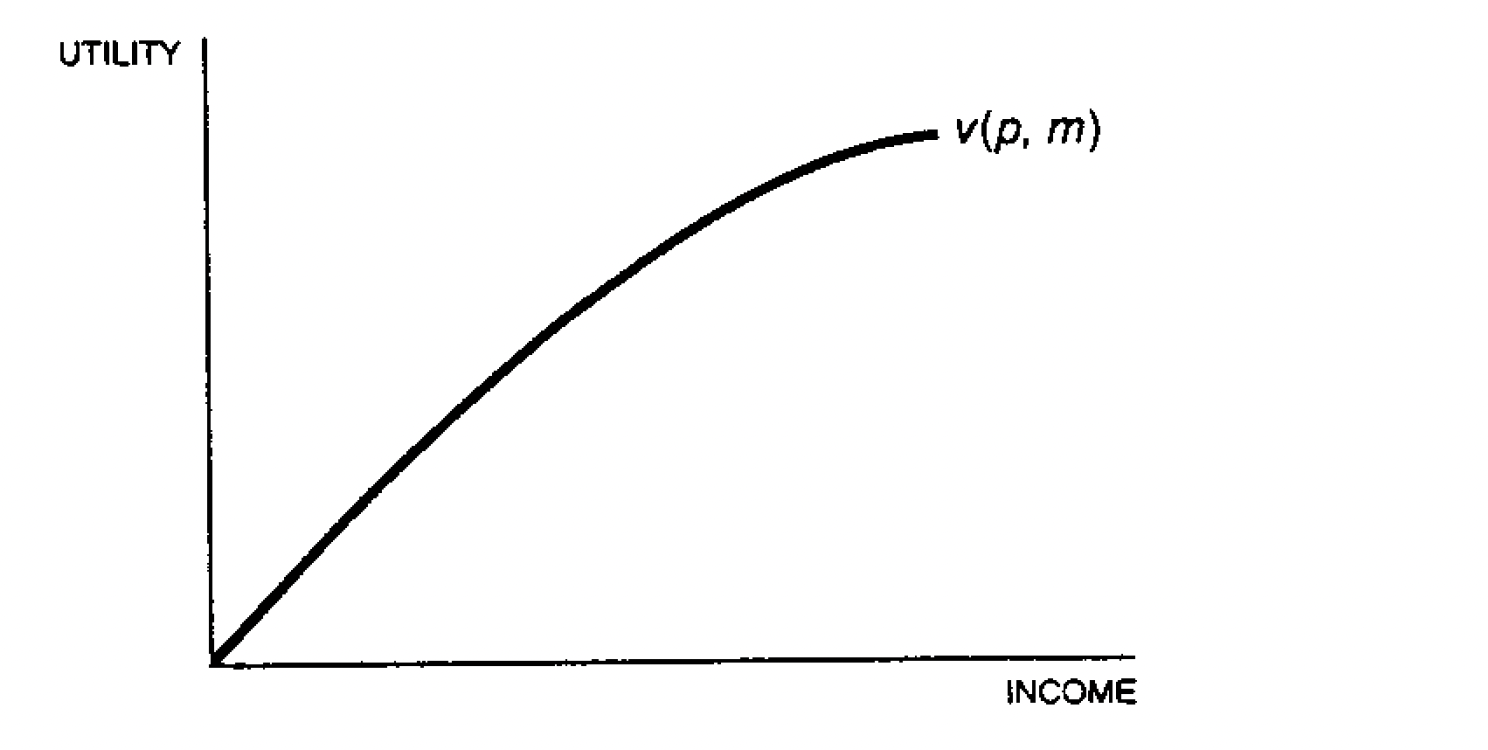
\includegraphics[width=0.7\textwidth]{img/fig7-3}
    \caption{$v^{-1}(\mathbf{p}, m) = e(\mathbf p , u)$}
\end{figure}

\block{Theorem: Expenditure Function}{
    Properties of the expenditure function: (類似 cost function)
    \begin{enumerate}
        \item $e(\mathbf p, u)$ is nondecreasing in $\mathbf p$. %; that is, if $\mathbf p^\prime \geq \mathbf p$, $v(\mathbf p^\prime, m) \leq v(\mathbf p, m)$. Similarly, $v(\mathbf p, m)$ is nondecreasing in $m$.
        \item $e(\mathbf p, u)$ is HD-1 in $\mathbf p$.
        \item $e(\mathbf p, u)$ is a concave in $\mathbf p$. %; that is $\{ \mathbf p :v(\mathbf p, m) \leq k \}$ is a convex set for all $k$.
        \item $e(\mathbf p, u)$ is continuous in $\mathbf p$ at all $\mathbf p \gg 0, m >0$.
        \item If $\mathbf h(\mathbf p, u)$ is the expenditure-minimizing bundle necessary to achieve utility level $u$ at prices $\mathbf p$, then $h_i(\mathbf p, u) = \frac{\partial e(\mathbf{p}, u)}{\partial p_i}$ for $i=1, \dots, k$ assuming the defivative exists and that $p_i > 0$.
    \end{enumerate}
}

\block{Definition: Hicksian Demand Function}{
    The function $h_i(\mathbf p , u)$ is called the Hicksian demand function. 
}
The Hicksian demand function tells us what consumtion bundle achieves a target level of utility and minimizes total expenditure. 
It is sometimes called a compensated demand function as it is constructed by varing prices and income so as to keep the consumer ata fixed level of utility.
Thus, income change are arragned to compensate for the price change.

Hicksian demand are not directly observable since they depend on utility, which is not directly observed.
$\mathbf{x}(\mathbf{p}, m)$ is called uncompensated demand function, Mashallian demand function.


\section{Some Important Identities}

Consider the utility maximization problem and expenditure minimization problem:
\begin{equation*}
    \begin{array}{rl}
        v(\mathbf p, m^*) = \max & \ u(\mathbf{x}) \\
        \text{s.t.} & \ \mathbf{px} \leq m
    \end{array} \iff
    \begin{array}{rl}
        e(\mathbf p, u^*) = \min & \ \mathbf{px} \\
        \text{s.t.} & \ u(\mathbf{x}) \geq u^*.
    \end{array}
\end{equation*}
The answers to these two problems should be the same $\mathbf x^*$.

\block{Theorem}{
    There's some important identities:
    \begin{enumerate}
        \item $e(\mathbf p, v(\mathbf p, m)) \equiv m$. \\
        The minimum expenditure necessary to reach utility $v(\mathbf p, m)$ is $m$. \\
        (在$\mathbf p$的價格下,要達到$v(\mathbf p, m)$效用水準的最小支出為$m$。)
        \item $v(\mathbf p, e(\mathbf p, u)) \equiv u$. \\
        The maximum utility from income $e(\mathbf p, u)$ is $u$. \\
        (在$\mathbf p$的價格及$e(\mathbf p, u)$所得水準之下,可達到的最高效用水準為$u$。)
        \item $x_i(\mathbf p, m)= h_i(\mathbf p, v(\mathbf p, m)).$ \\
        The Marshallian demand at income $m$ is the same as the Hicksian demand at utility $v(\mathbf p, m)$.\\
        (在$\mathbf p$價格、$m$所得水準之下的Marshallian demand等於在$\mathbf p$價格、$v(\mathbf p, m)$效用水準之下的Hicksian demand。)
        \item $h_i(\mathbf p, u) = x_i(\mathbf p, e(\mathbf p, u))$. \\
        The Hicksian demand at utility $u$ is the same as the Marshallian demand at income $e(\mathbf p, u)$.\\
        (在$\mathbf p$價格、$u$效用水準之下的Hicksian demand等於在$\mathbf p$價格、$e(\mathbf p, u)$所得水準之下的Marshallian demand。)
    \end{enumerate}
    $\implies$ Any demanded bundle can be expressed either as the solution to the utility maximization problem or the expenditure minimization problem.
}

\block{Theorem: Roy’s Identities}{
    If $\mathbf x(\mathbf p,m)$ is the Marshallian demand function, then
    \[
        x_i(\mathbf{p}, m) = -\frac{\frac{\partial v (\mathbf{p}, m)}{\partial p_i}}{\frac{\partial v (\mathbf{p}, m)}{\partial m}}
        \quad   \text{for} \ i = 1, \dots, k.
    \]
    \pf{
    Suppose that $\mathbf x^*$ yields a maximal utility of $u^*$ at $(\mathbf p^*, m^*)$. We know from the identities that
    \[
    \mathbf x^* (\mathbf p^*, m^*)
    =
    \mathbf h^* (\mathbf p^*, u^*).
    \]

    From another one of the fundamental identities, we also know that
    \[
        u^* = v(\mathbf p, e(\mathbf p, u^*)).
    \]
    This identity says that no matter what prices are, if you give the consumer the minimal income to get utility $u^*$ at those prices, then the maximal utility he can get is $u^*$.
        
    Since this is an identity we can differentiate it with respect to $p_i$ to get
    \begin{gather*}
        0=
        \frac{\partial v(\mathbf{p^*}, m^*)}{\partial p_i} +
        \frac{\partial v(\mathbf{p^*}, m^*)}{\partial m}
        \frac{\partial e(\mathbf{p^*}, u^*)}{\partial p_i} \\
        \implies
        \mathbf x^* (\mathbf p^*, m^*)
        \equiv
        \mathbf h^* (\mathbf p^*, u^*)
        \equiv
        \frac{\partial e(\mathbf{p^*}, u^*)}{\partial p_i}
        \equiv
        -\frac{\frac{\partial v (\mathbf{p}, m)}{\partial p_i}}{\frac{\partial v (\mathbf{p}, m)}{\partial m}}.
    \end{gather*}
    Since this identity is satisfied for al $(\mathbf p^*, \mathbf m^* )$ and since $\mathbf x^* = \mathbf x(\mathbf p^*, m^*)$, the result is proved.}
}

\block{Theorem: Roy's Identities (Continue)}{
    \pf{
    The utility function is given by
    \[
        v(\textbf p, m) \equiv 
        u(\textbf x (\textbf p, m))
        \quad \dots \ (1)
    \]
        
    If we differentiate this with respect to $p_j$, we find    
    \[
        \frac{\partial v (\mathbf p, m)}{\partial p_j}
        =
        \sum_{i=1}^k
        \frac{\partial u (\mathbf x)}{\partial x_i}
        \frac{\partial x_i}{\partial p_j}
        \quad \dots \ (2)
    \]
        
    Since $\textbf x (\textbf p, m)$ is the demand function, it satisfies the first-order conditions for utility maximization. Substituting the first-order conditions into expression $(2)$ gives
    \[
        \frac{\partial v (\mathbf p, m)}{\partial p_j}
        =
        \sum_{i=1}^k
        \lambda p_i
        \frac{\partial x_i}{\partial p_j}
        \quad \dots \ (3)
    \]
    The demand functions also satisfy the budget constraint $\textbf p\textbf x (\textbf p, m) \equiv m$. Differentiating this identity with respect to $p_j$, we have
    \[
        x_j(\mathbf p, m)+
        \sum_{i=1}^{k}p_i
        \frac{\partial x_i}{\partial p_j}
        =0
        \quad \dots \ (4)
    \]
        
    Substitute $(4)$ into $(3)$ to find
    \[
        \frac{\partial v (\mathbf p, m)}{\partial p_j} = 
        -\lambda x_j(\mathbf p, m)
        \quad \dots \ (5)
    \]
        
    Now we differentiate $(1)$ with respect to $m$ to find
    \[
        \frac{\partial v (\mathbf p, m)}{\partial m}
        =
        \sum_{i=1}^k
        \lambda p_i
        \frac{\partial x_i}{\partial m}
        \quad \dots \ (6)
    \]
        
    Differentiating the budget constraint with respect to $m$, we have    
    \[
        \sum_{i=1}^k
        p_i
        \frac{\partial x_i}{\partial m}
        =1
        \quad \dots \ (7)
    \]
        
    Substituting $(7)$ into $(6)$ gives us    
    \[
        \frac{\partial v (\mathbf p, m)}{\partial m}
        = \lambda
    \]
        
    This equation simply says that the Lagrange multiplier in the first-order condition is the marginal utility of income. Combining $(4)$ and $(7)$ gives us Roy's identity.
    }
}


\section{The Money Metric Utility Function}



\block{Definition: Money Metric Utility Function}{
    How much money would a given consumer need at the prices $\mathbf p$ to be as well off as he could by consuming the bundle $\mathbf x$.
    (在價格$\mathbf p$ 之下,選擇和既有消費組合$\mathbf x$至少一樣好的效用水準的最小支出。)
    \begin{align*}
        \underset{\mathbf{z}}{\min} &\ \mathbf{pz} \\
        \text{s.t.} &\ u(\mathbf{z}) \geq u(\mathbf{x})
    \end{align*}    
    Also known as "minimum income function" or "direct compensation function". 
    An alternative definition is 
    \[
        m(\mathbf{p, x}) \equiv e(\mathbf{p}, u(\mathbf{x})).
    \]
}
\begin{itemize}
    \item If $\mathbf{x}$ is fixed $\to$ $u(\mathbf{x})$ is fixed $\to$ $m(\mathbf{p, x})$ behaves exactly like an expenditure function: \\
    monotonic, homogeneous, concave in $\mathbf p$, and os on.
    \item If $\mathbf{p}$ is fixed $\to$ $m(\mathbf{p, x})$ is an utility function:
\end{itemize}


\block{Definition: Money Metric Indirect Utility Function}{
    \[
        \mu(\mathbf{p}; \mathbf{q}, m) = e(\mathbf{p}, v(\mathbf{q}, m)).
    \]
    $\mu(\mathbf{p}; \mathbf{q}, m)$ measures how much money one would need at prices $\mathbf{p}$ to be as well off as one would be facing prices $\mathbf q$ and having income $m$.
    (在價格$\mathbf{p}$ 之下,支出要達到多少才可以達到 $v(\mathbf q, m)$ 的效用水準。) 
}
$\mu(\mathbf{p}; \mathbf{q}, m)$ behave like an expenditure function with respect to $\mathbf{p}$, but now it behaves like an indirect utility function with respect to $\mathbf q$ and $m$, since it is simply a monotonic transformation of an indirect utility function.
\begin{itemize}
    \item If $v(\mathbf{q}, m)$ is fixed $\to$ $\mu(\mathbf{p}; \mathbf{q}, m)$ is an expenditure function
    \item If $\mathbf{p}$ is fixed $\to$ $\mu(\mathbf{p}; \mathbf{q}, m)$ is an (indirect) utility function
\end{itemize}

\block{Example: Cobb-Douglas utility function}{

}
\block{Example: The CES utility function}{

}